% Options for packages loaded elsewhere
% Options for packages loaded elsewhere
\PassOptionsToPackage{unicode}{hyperref}
\PassOptionsToPackage{hyphens}{url}
\PassOptionsToPackage{dvipsnames,svgnames,x11names}{xcolor}
%
\documentclass[
  letterpaper,
  DIV=11,
  numbers=noendperiod]{scrartcl}
\usepackage{xcolor}
\usepackage{amsmath,amssymb}
\usepackage{setspace}
\setcounter{secnumdepth}{-\maxdimen} % remove section numbering
\usepackage{iftex}
\ifPDFTeX
  \usepackage[T1]{fontenc}
  \usepackage[utf8]{inputenc}
  \usepackage{textcomp} % provide euro and other symbols
\else % if luatex or xetex
  \usepackage{unicode-math} % this also loads fontspec
  \defaultfontfeatures{Scale=MatchLowercase}
  \defaultfontfeatures[\rmfamily]{Ligatures=TeX,Scale=1}
\fi
\usepackage{lmodern}
\ifPDFTeX\else
  % xetex/luatex font selection
\fi
% Use upquote if available, for straight quotes in verbatim environments
\IfFileExists{upquote.sty}{\usepackage{upquote}}{}
\IfFileExists{microtype.sty}{% use microtype if available
  \usepackage[]{microtype}
  \UseMicrotypeSet[protrusion]{basicmath} % disable protrusion for tt fonts
}{}
\makeatletter
\@ifundefined{KOMAClassName}{% if non-KOMA class
  \IfFileExists{parskip.sty}{%
    \usepackage{parskip}
  }{% else
    \setlength{\parindent}{0pt}
    \setlength{\parskip}{6pt plus 2pt minus 1pt}}
}{% if KOMA class
  \KOMAoptions{parskip=half}}
\makeatother
% Make \paragraph and \subparagraph free-standing
\makeatletter
\ifx\paragraph\undefined\else
  \let\oldparagraph\paragraph
  \renewcommand{\paragraph}{
    \@ifstar
      \xxxParagraphStar
      \xxxParagraphNoStar
  }
  \newcommand{\xxxParagraphStar}[1]{\oldparagraph*{#1}\mbox{}}
  \newcommand{\xxxParagraphNoStar}[1]{\oldparagraph{#1}\mbox{}}
\fi
\ifx\subparagraph\undefined\else
  \let\oldsubparagraph\subparagraph
  \renewcommand{\subparagraph}{
    \@ifstar
      \xxxSubParagraphStar
      \xxxSubParagraphNoStar
  }
  \newcommand{\xxxSubParagraphStar}[1]{\oldsubparagraph*{#1}\mbox{}}
  \newcommand{\xxxSubParagraphNoStar}[1]{\oldsubparagraph{#1}\mbox{}}
\fi
\makeatother


\usepackage{longtable,booktabs,array}
\usepackage{calc} % for calculating minipage widths
% Correct order of tables after \paragraph or \subparagraph
\usepackage{etoolbox}
\makeatletter
\patchcmd\longtable{\par}{\if@noskipsec\mbox{}\fi\par}{}{}
\makeatother
% Allow footnotes in longtable head/foot
\IfFileExists{footnotehyper.sty}{\usepackage{footnotehyper}}{\usepackage{footnote}}
\makesavenoteenv{longtable}
\usepackage{graphicx}
\makeatletter
\newsavebox\pandoc@box
\newcommand*\pandocbounded[1]{% scales image to fit in text height/width
  \sbox\pandoc@box{#1}%
  \Gscale@div\@tempa{\textheight}{\dimexpr\ht\pandoc@box+\dp\pandoc@box\relax}%
  \Gscale@div\@tempb{\linewidth}{\wd\pandoc@box}%
  \ifdim\@tempb\p@<\@tempa\p@\let\@tempa\@tempb\fi% select the smaller of both
  \ifdim\@tempa\p@<\p@\scalebox{\@tempa}{\usebox\pandoc@box}%
  \else\usebox{\pandoc@box}%
  \fi%
}
% Set default figure placement to htbp
\def\fps@figure{htbp}
\makeatother





\setlength{\emergencystretch}{3em} % prevent overfull lines

\providecommand{\tightlist}{%
  \setlength{\itemsep}{0pt}\setlength{\parskip}{0pt}}



 


\KOMAoption{captions}{tableheading}
\makeatletter
\@ifpackageloaded{caption}{}{\usepackage{caption}}
\AtBeginDocument{%
\ifdefined\contentsname
  \renewcommand*\contentsname{Table of contents}
\else
  \newcommand\contentsname{Table of contents}
\fi
\ifdefined\listfigurename
  \renewcommand*\listfigurename{List of Figures}
\else
  \newcommand\listfigurename{List of Figures}
\fi
\ifdefined\listtablename
  \renewcommand*\listtablename{List of Tables}
\else
  \newcommand\listtablename{List of Tables}
\fi
\ifdefined\figurename
  \renewcommand*\figurename{Figure}
\else
  \newcommand\figurename{Figure}
\fi
\ifdefined\tablename
  \renewcommand*\tablename{Table}
\else
  \newcommand\tablename{Table}
\fi
}
\@ifpackageloaded{float}{}{\usepackage{float}}
\floatstyle{ruled}
\@ifundefined{c@chapter}{\newfloat{codelisting}{h}{lop}}{\newfloat{codelisting}{h}{lop}[chapter]}
\floatname{codelisting}{Listing}
\newcommand*\listoflistings{\listof{codelisting}{List of Listings}}
\makeatother
\makeatletter
\makeatother
\makeatletter
\@ifpackageloaded{caption}{}{\usepackage{caption}}
\@ifpackageloaded{subcaption}{}{\usepackage{subcaption}}
\makeatother
\usepackage{bookmark}
\IfFileExists{xurl.sty}{\usepackage{xurl}}{} % add URL line breaks if available
\urlstyle{same}
\hypersetup{
  pdftitle={On the Effects of Government Medical Spending and Health Personnel On HIV Spread},
  colorlinks=true,
  linkcolor={blue},
  filecolor={Maroon},
  citecolor={Blue},
  urlcolor={Blue},
  pdfcreator={LaTeX via pandoc}}


\title{On the Effects of Government Medical Spending and Health
Personnel On HIV Spread}
\author{}
\date{}
\usepackage{setspace}
\singlespacing
\usepackage[left=2cm, right=2cm, top=2cm, bottom=2cm]{geometry}
\begin{document}
\maketitle


David Jiang

\subsection{Introduction}\label{introduction}

The motivation behind this analysis is to investigate whether it is
worthwhile for a country to invest more into the health sector to reduce
the spread of HIV. The dataset used for this purpose is the World Health
Organization's (WHO) Global Health Observatory's (GHO) data. The focus
of the data obtained from this dataset will be on HIV data, health
personnel data, and economic data, specifically economic data as a whole
and for health/medical related uses. The question is whether
health/medical spendings and personnel affect the spread of HIV, and if
so, by how much. The hypothesis is that these factors do indeed affect
the spread of HIV, especially the spendings. The result of this analysis
can help governments determine how much they should spend on the medical
sector if they wish to reduce the spread of HIV in their country.

\subsection{Methods}\label{methods}

First, a general list of indicators were queried using WHO's GBO's API.
Then, the list was inspected and indicators useful for analyzing the key
question were selected. The indicators were chosen if they were related
to government spending or to health personnel. Since there is a lot of
missing data for personnel indicators, only indicators for the three
core personnel types were chosen, aside from government medical spending
indicators. These included doctors, nurses and midwives, and
pharmacists. Furthermore, to keep things proportionate, the number of
such personnel per 10,000 population was used instead of total count, as
some countries may have less overall but the same in proportion. \\
The data for number of new HIV infections and domestic general government
health expenditure as percentage of general government expenditure were
obtained directly from WHO's GBO via the API. However, API queries for
other indicators of interest responded successfully (status code 200),
but contained no data. As such, the information has been retrieved in
the form of CSV files. The data's features were then inspected, and all
unnecessary columns and columns with no data were dropped. Unnecessary
columns included ones such as redundant information (there were several
columns giving the same date/time information) and identifiers (IDs).
This left only the country, region, year, and indicators. \\
After merging
the data into one data frame using left joins, there were 5095 entries
total with 8 columns. Each row contains information on the indicators
for one country for one specific year. Note that the regions include but
are not the same as the continents. Specifically, the regions are:
Eastern Mediterranean, Africa, Europe, Americas, Western Pacific, and
South-East Asia. \\
Then, to understand the global trend of the data, a
plot contrasting the spendings, new cases, and year of each country was
made. This plot can be seen as an interactive visualization on the
webpage as Figure 1, this is not to be confused with Figure 1 in this
report. \\
Finally, to deal with missing data, much analysis was performed,
including via linear regression, to see whether each indicator should be
dropped. The analysis for this is mostly checking the statistical significance of
each indicator when fitting them to a linear model. The results will be
explained more in depth in the results section. \\
I then decided to
perform a linear imputation of the missing data, as there would be a
strong lack of training data otherwise. A more detailed explanation for
doing this can be seen in the results section.

Then the data was split via by an 80 to 20 ratio of training/validation
to testing, and then modeled by XGBoost, linear regression, and random
forest regressor. The models will use the number of new cases
(new\_cases) as the response variable and the health expense and
personnel indicators as predictors. Each model has four variants,
differing by the indicators used in their training. There is one with
all indicators, one with nurse count dropped, one with the health
expense dropped, and one where the core personnel count was aggregated
into one total value instead of spread over several. The reason for this
was to deal with potential multicollinearity between the amounts of
different personnel. \\
The hyperparameters will be tuned via a 5 fold
cross validation. \\
The XGBoost regressor is a model that performs
gradient boosting, parallelised via trees. It includes regularization
and many other optimization methods to fit to the data while trying to
avoid overfitting. Key hyperparameters of this model include the number
of estimators, the depth of the tree, the learning rate, and possible
early stops. \\
The random forest regressor uses the average of multiple
decision trees to give a value to a point. Since each decision tree was
made by subsetting different features at each split, they are different
from each other. Key hyperparameters include the maximum number of
features to consider, the minimum number of samples per leaf, and the
number of estimators. \\
The linear regressor is the baseline model used.
It uses the ordinary least squares method to minimize the residual sum
of squares between the observed data and the predicted values. \\
Key statistics to be used in comparing the models and testing significance
of features include the R\(^2\), adjusted R\(^2\), AIC, and RMSE.
Overall, to compare the three types of models, RMSE, R\(^2\), and
will be used.

\subsection{Results}\label{results}

The first thing to analyze is the missing data. To do this, Figure 1 below was
generated. Based on the figure, there are quite a lot of missing values,
with there being around 40-50\% of the entries being missing for the
health personnel. On top of that, there are around 26\% of entries
missing the new HIV cases value. With this in mind, I then checked the
missing values based on year instead. From there, I noticed that years
1990-1999 have extremely high proportion of missing, plus the
expenditure values for 2024. With this in mind, it was decided that the
years 1990-1999 and 2024 would be dropped. Since it is impossible to
analyze the years where a country has no data on the response variable,
number of new cases, entries with no data on new cases were dropped.

\begin{figure}[H]

{\centering \pandocbounded{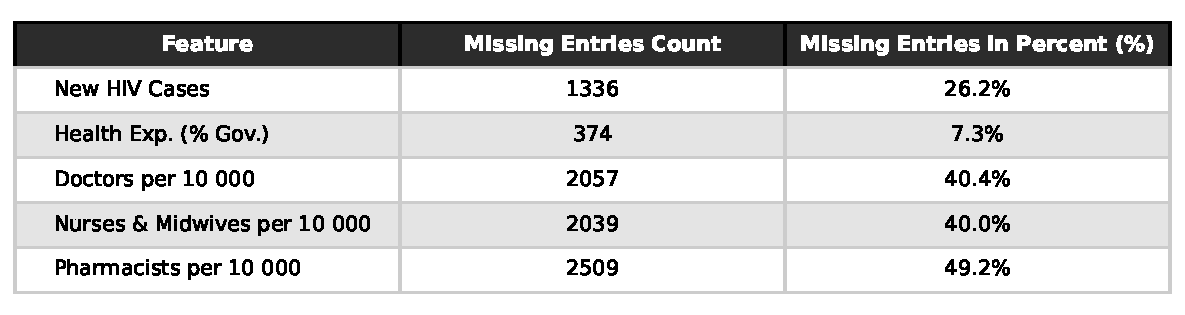
\includegraphics[keepaspectratio]{final_files/figure-pdf/cell-8-output-1.pdf}}

}

\caption{Missing entries for each feature}

\end{figure}%

After checking the proportion of data still missing, Figures 2 and 3
reveal that the main issue in the high amount of missing data for the
features remain. Figure 3 in particular shows the higher number of
missing data in Africa.

\begin{figure}[H]

{\centering \pandocbounded{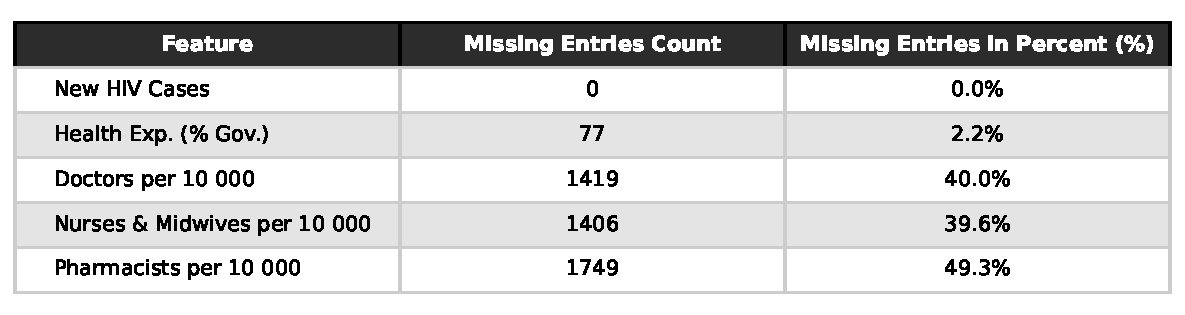
\includegraphics[keepaspectratio]{final_files/figure-pdf/cell-10-output-1.pdf}}

}

\caption{Missing entries for each feature, after dropping
entries with missing new HIV cases, as well as filtering for years
2000-2023}

\end{figure}%

\begin{figure}[H]

{\centering \pandocbounded{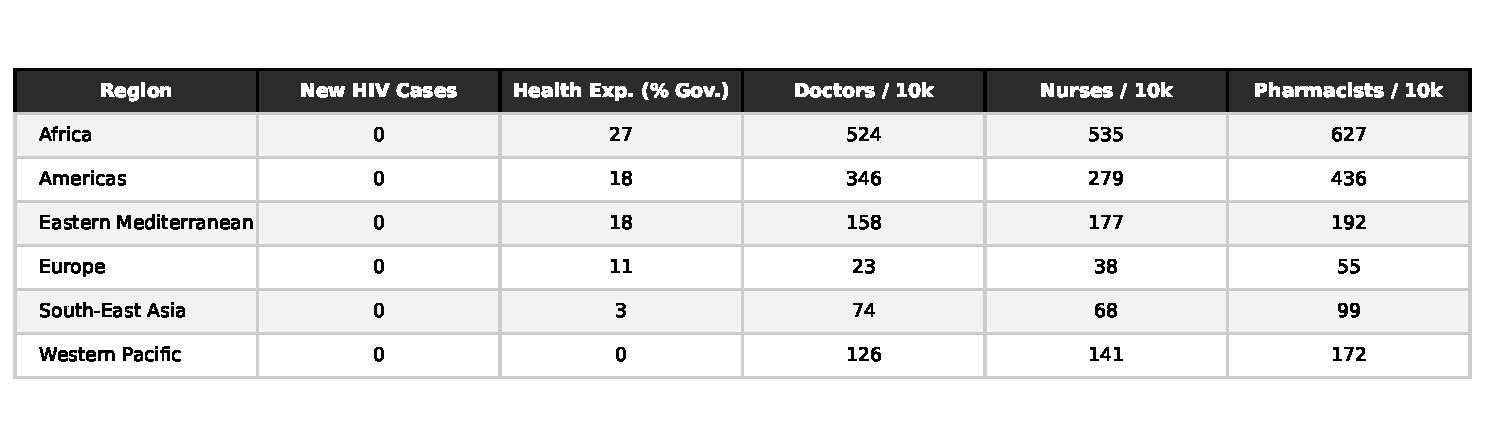
\includegraphics[keepaspectratio]{final_files/figure-pdf/cell-11-output-1.pdf}}

}

\caption{Number of missing entries for each region, for each
feature}

\end{figure}%

At this point, I realized that Venezuela and Saint Kitts
and Nevis in particular are missing all of their data on pharmacists, as
such, the decision was made to exclude them from the analysis. I then
decided to fit several linear regression models to check whether any of the features could
be dropped due to low significance.
The result was that when any of the personnel features are dropped,
government health expenses becomes no longer significant at the 0.05
level. However, in the full model, all features appear to be significant
at the 0.05 level. \\
Comparing the r-squared, there does not appear to be
any significant difference for any of the models, with all of them around 0.05-0.07. Furthermore, in the
last model, the one with only personnel data, both the nurse/midwives
and pharmacist features are no longer significant at the 0.05 level.
On top of that, the proportion of nurses seems to universally have the
smallest effect on the spread of HIV in comparison to the other
personnel. While it makes sense that the coefficients of each personnel
is negative, indicating that more personnel leads to a reduced spread,
the health expense is always positive, which indicates that more
spending leads to a greater spread, this is counterintuitive, but can be explained by low efficiency spending. 

\begin{figure}[H]

{\centering \pandocbounded{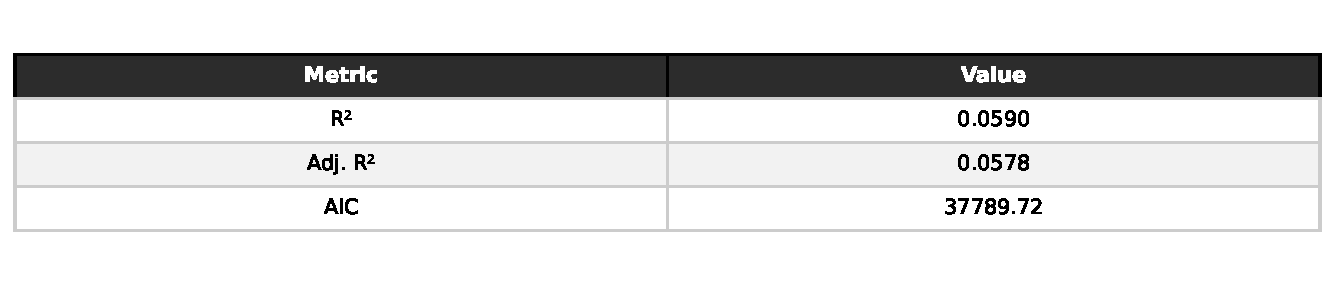
\includegraphics[keepaspectratio]{final_files/figure-pdf/cell-15-output-1.pdf}}

}

\caption{Table showing the metrics of a linear regression
model that uses the total personnel across the three categories plus the
health expense.}

\end{figure}%

From here, I then decided to impute linearly much of the originally
missing values and refit the models. The imputations are done on a
country by country basis, using the most recent existing years with data
to impute. In terms of the r-squared, proportionally speaking, removing
the doctor count reduces the performance to a more noticeable degree than
removing other features. Also notably, with the exception of
nurse/midwife and pharmacist counts, other features are shown as
non-significant in any model when using the imputed data. Even
pharmacist count was only statistically insignificant when health
expenditure was excluded as a feature. Though there is a decrease in
r-squared when compared to the models not using the imputed dataset. The four subsets of features were chosen based on this.

Figure 2 on the webpage show the result of the modeling. When comparing the three types of models, we see
that the baseline linear regression performs quite poorly in comparison
to the random forest and XGBoost models when using either the RMSE or
R\(^2\) as the metric. It is also evident that among the four variants
of each model, aggregating the personnel information causes the model to
perform far more poorly, which indicates that the information lost from
the aggregation has a greater impact than the reduction of
multicollinearity from merging the features into one. Aside from that,
the models with all features also performs a touch better than when
removing the nurse proportion or removing the health expenses, when
using either metrics, which makes sense considering such a model would
have more information. \\
Based on the residual plot show in Figure 3 on the webpage, we see that the linear regression model ends up over
predicting the values by a large margin, while the other two have much
less extreme values. The systematic patterns of the errors also
indicates that a transformation, perhaps via the log function, would
help improve the models. Regardless, each model struggles to predict
large values. From the predicted versus actual plot shown in Figure 4 on
the webpage, we can see that the XGB model tends to do slightly better
than the random forest on larger values, but appears to over predict the
smaller values, as can be seen by the cluster above the dashed line near
0. The dashed line indicates where the points would be if the prediction
and actual value coincided, meaning that the closer the value is to the
dashed line, the more accurate that prediction was. \\

\begin{figure}[H]

{\centering \pandocbounded{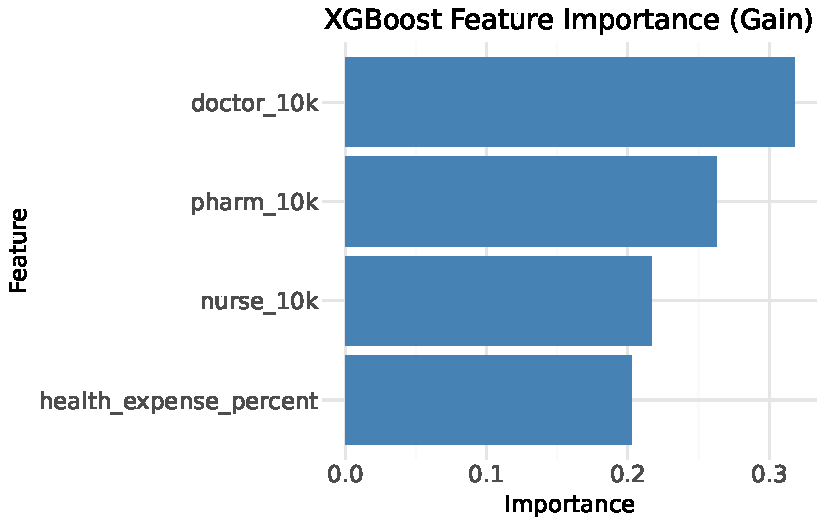
\includegraphics[keepaspectratio]{final_files/figure-pdf/cell-24-output-1.pdf}}

}

\caption{Feature importances for the XGB model.}

\end{figure}%

Then, Figure 5 was
plotted to show the feature importances given by the XGB model. We can
see from here that the health expenditure proportion has the least
impact on the model's predictions, while the proportion of doctors,
pharmacists, and nurses/midwives have, in that order, the most to least
importance for the predictions. \\

\begin{figure}[H]

{\centering \pandocbounded{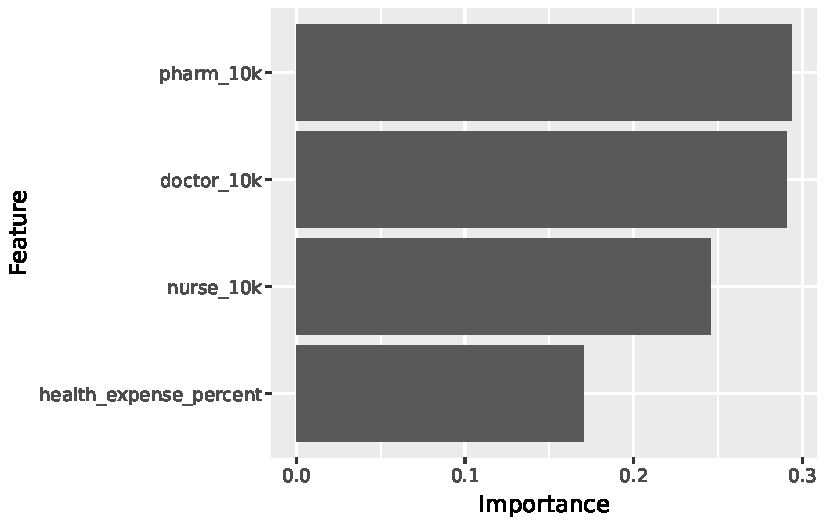
\includegraphics[keepaspectratio]{final_files/figure-pdf/cell-25-output-1.pdf}}

}

\caption{Feature importances for the Random Forest model.}

\end{figure}%

Figure 6, generated from the random
forest model, shows a similar trend in that the least important feature
is the health expense, though for the random forest, the proportion of
doctors is slightly less important, putting it as the second most
important by a narrow margin compared to the the proportion of
pharmacists. \\
The rankings for the XGB model makes sense, and the random
forest model's does too, to a lesser extent. Intuitively, the proportion
of doctors to population is an indicator of a country's medical spending
and extensiveness of their health infrastructure. However, less
intuitively, the random forest ranks pharmacists roughly just as
importantly as doctors. This perhaps has to do with a nation's wealth
and scientific development of their medical field. Pharmacists are more
useful when a nation has the wealth to invest in drug research,
purchase, and/or development. When these are not present, a country
would likely not see as much of a point in investing into more
pharmacists, preferring to put the spendings into other things. Lastly,
the low ranking of the importance of health expenses is likely because
health expenses encompasses too many items, and as such has too much
noise in the data for the model to make good use of it, in comparison to
the number of doctors. Furthermore, a sizeable portion of a nation's
health spendings are likely on these 3 core personnel, therefore much of the
information is included already in other features, making health
expenses less informative. \\
Since keeping all features results in a better
model both based on RMSE and R\(^2\), as well as that the random forest
model performs slightly better than the XGB model by both metrics, the
test set was ultimately run on the random forest model, yielding a test
RMSE of around 14573 and a test R\(^2\) of around 0.7872, in contrast to
the RMSE of about 16734 and R\(^2\) of about 0.8136 it achieved on the
training set. The closeness of the R\(^2\) and the smaller RMSE
indicates that this model performs quite well on the test set as well.\\
Out of concern for multicollinearity between the personnel data, a model that aggregates personnel data into a total core personnel per 10 000 population will also be examined.

\subsection{Conclusion}\label{conclusion}

Ultimately, the results of the models indicate that to reduce the spread
of HIV, governments should focus their health sector expenditure on
personnel, especially doctors and pharmacists. While HIV can indeed
spread via births, it appears the the effect of nurses and midwives are
limited in the bigger picture. This analysis, however, is limited by the
fact that the linear regression model performed quite poorly, as such, I
am unable to conclude as to a rough number of how each 1 personnel
increase would affect the spread. \\
The missing data also reduces the
accuracy these models would have in the real world, as around 40-50\% of
the data were imputed linearly. Thus, should the real world trends not
follow a linearly pattern, these imputations would cause the models to
give results that are inconsistent with the real world.
Furthermore, two countries, Venezuela and Saint Kitts and Nevis, were excluded from the data due to a complete lack of data on the number
of pharmacists. This lack prevented even imputations, resulting in the
models being less applicable to their countries. \\
A log transformation of
the response variables would have possibly also improved the models.
However, this would reduce the interpretability of the models, which was
why it was not performed here.

\end{document}
